%% REPLACE sXXXXXXX with your student number
\def\studentNumber{s2196789}


%% START of YOUR ANSWERS
%% Add answers to the questions below, by replacing the text inside the brackets {} for \youranswer{ "Text to be replaced with your answer." }. 
%
% Do not delete the commands for adding figures and tables. Instead fill in the missing values with your experiment results, and replace the images with your own respective figures.
%
% You can generally delete the placeholder text, such as for example the text "Question Figure 2 - Replace the images ..." 
%
% There are 19 TEXT QUESTIONS (a few of the short first ones have their answers added to both the Introduction and the Abstract). Replace the text inside the brackets of the command \youranswer with your answer to the question.
%
% There are also 3 "questions" to replace some placeholder FIGURES with your own, and 3 "questions" asking you to fill in the missing entries in the TABLES provided. 
%
% NOTE! that questions are ordered by the order of appearance of their answers in the text, and not by the order you should tackle them. Specifically, you cannot answer Questions 2, 3, and 4 before concluding all of the relevant experiments and analysis. Similarly, you should fill in the TABLES and FIGURES before discussing the results presented there. 
%
% NOTE! If for some reason you do not manage to produce results for some FIGURES and TABLES, then you can get partial marks by discussing your expectations of the results in the relevant TEXT QUESTIONS (for example Question 8 makes use of Table 1 and Figure 2).
%
% Please refer to the coursework specification for more details.


%% - - - - - - - - - - - - TEXT QUESTIONS - - - - - - - - - - - - 

%% Question 1:
\newcommand{\questionOne} {
\youranswer{model cannot be well generalized from the original data set to another new data set.}
}

%% Question 2:
\newcommand{\questionTwo} {
\youranswer{will make overfitting worse.}
}

%% Question 3:
\newcommand{\questionThree} {
\youranswer{dropout and L1/L2 regluation will mitigate overfitting problem and improve the performance of the trained model.}
}

%% Question 4:
\newcommand{\questionFour} {
\youranswer{overfitting is an important problem that we need to keep in mind when we train models despite what methods we used}
}

%% Question 5:
\newcommand{\questionFive} {
\youranswer{there is another model $F'$ which makes larger error rate than the given model $F$ on the training example, but the error rate of $F'$'s is smaller than $F$ in the entire distribution.}
}

%% Question 6:
\newcommand{\questionSix} {
\youranswer{There are many reasons that cause the  overfitting, including too much parameters or too high complexity of the model, or overtraining the model.
We can identify it is happening by noticing that the model makes more mistakes on training data but fewer mistakes on unseen future data.}
}

%% Question 7:
\newcommand{\questionSeven} {
\youranswer{it shows the error curve on the training and validation set of EMNIST dataset. The error rate decreases on the training set by going through each epoch. However, the error rate of validation set decreased and reached its minimum at approximately epoch 15, then increases after each epoch. The reason behind this is that our model fits the noise in the training data set which will not re-appear in the validation data set. There is another point which is noticeable. We could find that the slop of error and accuracy curve at first few epoch is steep. It is because at first few epoch the error is large which makes the model learn fast.}
}

%% Question 8:
\newcommand{\questionEight} {
\youranswer{as we increase the hidden units per layer, the generalization gap increases as well. The validation accuracy also increases, but according to the curvature of validation accuracy, even if the model with 128 hidden units(green line) has higher accuracy, it decreases faster after each epoch despite it increasing in the training set, which makes overfitting even worse. We could make a presumption that if we continue train the model with more epoch, the accuracy will become lower than that of 32 or 64 hidden units.}
}

%% Question 9:
\newcommand{\questionNine} {
\youranswer{From above figures we could find out that by adding hidden units up to 64 will kind of increase the validation accuracy, but when we add hidden units up to 128 there will be a dramatic increasing in generalization gap which will make overfitting worse. Hence varying width affects the
does not always results in a consistent way. In the case of 32 hidden units, it might be underfitting for a classifier with 47 different classes. However if there are 128 hidden units, the model becomes overfitting to the training set.}
}

%% Question 10:
\newcommand{\questionTen} {
\youranswer{there is no obvious differences between different depths on training set, but on validation set depth2 has the highest generalization gap. The model with 3 hidden layers has the best performance with highest validation accuracy and smallest generalization gap.}
}

%% Question 11:
\newcommand{\questionEleven} {
\youranswer{The results are not expected or match well with the prior knowledge because increasing depth does not affect the model's performance on training set, and it makes the generalization gap smaller. In other words, it mitigates the overfitting problem. According to prior knowledge, model with too much complexity should be more likely to overfitting to the training set. }
}

%% Question 12:
\newcommand{\questionTwelve} {
\youranswer{By comparing with two figures discussed previously, we could conclude that varying width and height changes the performance and overfitting in different way. If we keeping adding hidden units and make our model more complex, we will get the model overfitting, whereas adding the depth will kind of mitigate overfitting. However, by doing so also makes our model more complex and will get a larger generalization gap than that of model with a single hidden layer and small hidden units(32 and 64), which makes overfitting even worse.}
}

%% Question 13:
\newcommand{\questionThirteen} {
\youranswer{The main idea for L1/L2 regulation is that they aim to control the complexity of our model by adding penalties to loss function and penalize weight. In machine learning, we use gradient descend to train our model. If we add a regulation term to loss function, we make it not differentiable since it has absolute value, which means we add a constrain to loss function. The formula for L1 regulation is
\begin{align}
    L = E_{in}+\lambda\sum_{j}||w_{j}||
\end{align} 
L1 regulation is that it adds a penalty which is equal to the absolute value of the magnitude of coefficient. L1 regulation can produce sparsity, which most of weights in a model are 0. The hyperparameter for L1 regulation is $\lambda$ which controls the magnitude of L1 function. The formula for L2 regulation is
\begin{align}
    L = E_{in}+\lambda\sum_{j}||w_{j}||^{2}
\end{align} 
L2 regulation is that it adds a penalty which is equal to the square of the magnitude of coefficient. L2 regulation can alleviate overfitting. The hyperparameter for L2 regulation is $\lambda$ which performs the same function as in L1 regulation. 
}
}

%% Question 14:
\newcommand{\questionFourteen} {
\youranswer{
Our aim is to minimize loss function when it is constrained regulation. Consider that there are two parameters in weight matrix, $w_1$ and $w_2$. The point which optimized loss function is when the regulation function intersects with the contour of loss function. If we draw a function of L1, it will be a rectangular. Usually the contour of loss function will touch the L1 function at a corner, leading a sparsity solution. The function of L2 regulation is circular. We will always get small parameters(but nonzero) for weight when the contour of loss function touches the L2 function. Small parameters will make our model robust because they can fit in various data set. Large parameters are sensitive to various data set. In summary, both L1 and L2 regulation can address overfitting.
}
}

%% Question 15:
\newcommand{\questionFifteen} {
\youranswer{By comparing the validation accuracy and generalization gap of the baseline model and regularized models, we could find that the models implemented with dropout layer or L1/L2 penalty have higher validation accuracy and smaller generalization gap. Adjusting hyperparameter values also changes the performance of the model. In figure 4, it shows that the model has the best performance when the dropout value ranges between 0.4 and 0.6. And for weight decay value, the model performs poorly when the weight decay value is too large($10^-2$ or $10^-1$). We got the best overall results when L2 regulation was implemented individually. Its validation accuracy and generalization gap are obviously better than previous model which does not have overfitting problem. In combination of dropout and L1/L2 regulation, we found that implements dropout layers together with L1/L2 regulation does not improve the model's performance. To explain this phenomena, according to the function of L1/L2 regulation, we could assume that the weights in model with L1/L2 regulation are already regularized not to overfit the training set. If we drop out some weights based on this, it could decrease the accuracy of the model, but the generalization performance of the model is still good since it does not have overfiting problem. 
}
}

%% Question 16:
\newcommand{\questionSixteen} {
\youranswer{it can't fit well with ideal stochastic gradient operation and its approximation for the deep model could be enhanced}

}

%% Question 17:
\newcommand{\questionSeventeen} {
\youranswer{Dropout is compitable with Maxout activation function because Maxout  is locally linear. Unlike other activation functions such as ReLU or sigmoid, which constraints dropout model averaging, Maxout has better performance when trained with dropout by its property of piecewise linear function.
}
}

%% Question 18:
\newcommand{\questionEighteen} {
\youranswer{In the experiment the authors evaluated the Maxout model by testing it with four different dataset, MNIST, CIFAR-10, CIFAR-100, and SVHN, and comparing the test results with that of other methods. They conclude that the Maxout model together with dropout has the lowest test error. In addition, they also point out that the enhancement of test error is not from preprocessing or large models, but from the use of Maxout. The authors compare Maxout to rectifiers with the same processing by a set of cross-validation experiments and they find Maxout performs better than rectifiers}
}

%% Question 19:
\newcommand{\questionNineteen} {
\youranswer{Based on the results from reviewing of Maxout networks, we found that although Maxout can improve accuracy and minimize error for dropout, it may also cause overfitting problem in some extreme cases. Maxout is not always the best choice over other methods. In machine learning there are many complicated circumstances in which data are usually complex and unexpected. There are many methods we could use to mitigating overfitting such as dropout, L1/L2 regulation, but we need to pay attention to this problem because it happens frequently when we train models despite what methods we used}
}


%% - - - - - - - - - - - - FIGURES - - - - - - - - - - - - 

%% Question Figure 2:
\newcommand{\questionFigureTwo} {


\begin{figure}[t]
    \centering
    \begin{subfigure}{\linewidth}
        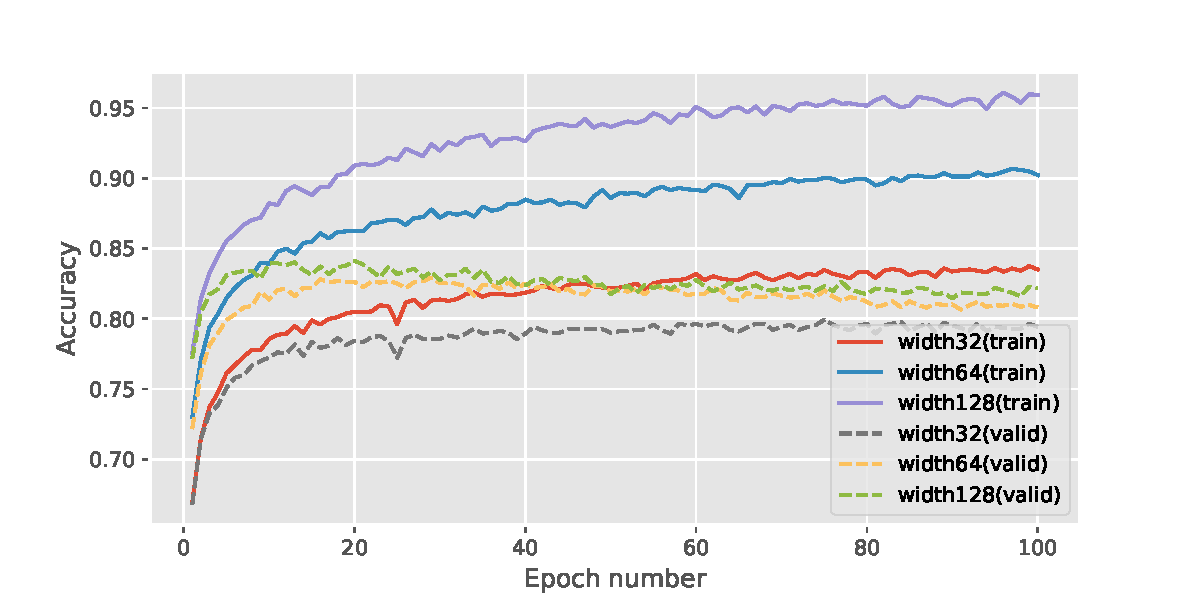
\includegraphics[width=\linewidth]{hidden_unit_acc.pdf}
        \caption{accuracy by epoch}
        \label{fig:width_acccurves}
    \end{subfigure} 
    \begin{subfigure}{\linewidth}
        \centering
        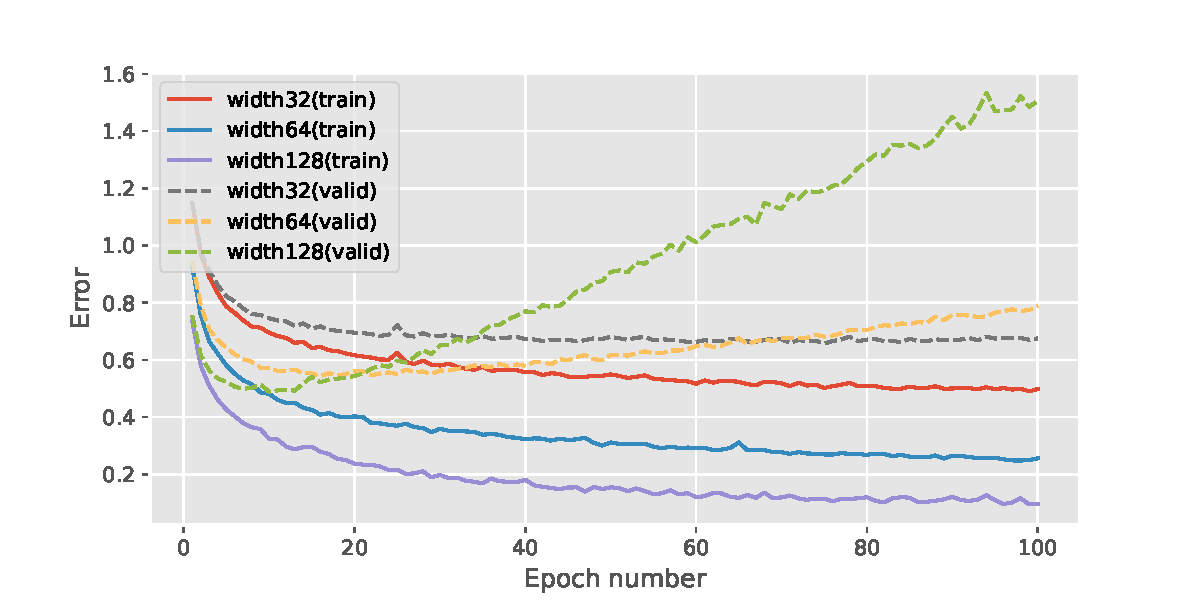
\includegraphics[width=\linewidth]{hidden_unit_err.pdf}
        \caption{error by epoch}
        \label{fig:width_errorcurves}
    \end{subfigure} 
    \caption{Training and validation curves in terms of classification accuracy (a) and cross-entropy error (b) on the EMNIST dataset for different network widths.}
    \label{fig:width}
\end{figure} 


}

%% Question Figure 3:
\newcommand{\questionFigureThree} {


\begin{figure}[t]
    \centering
    \begin{subfigure}{\linewidth}
        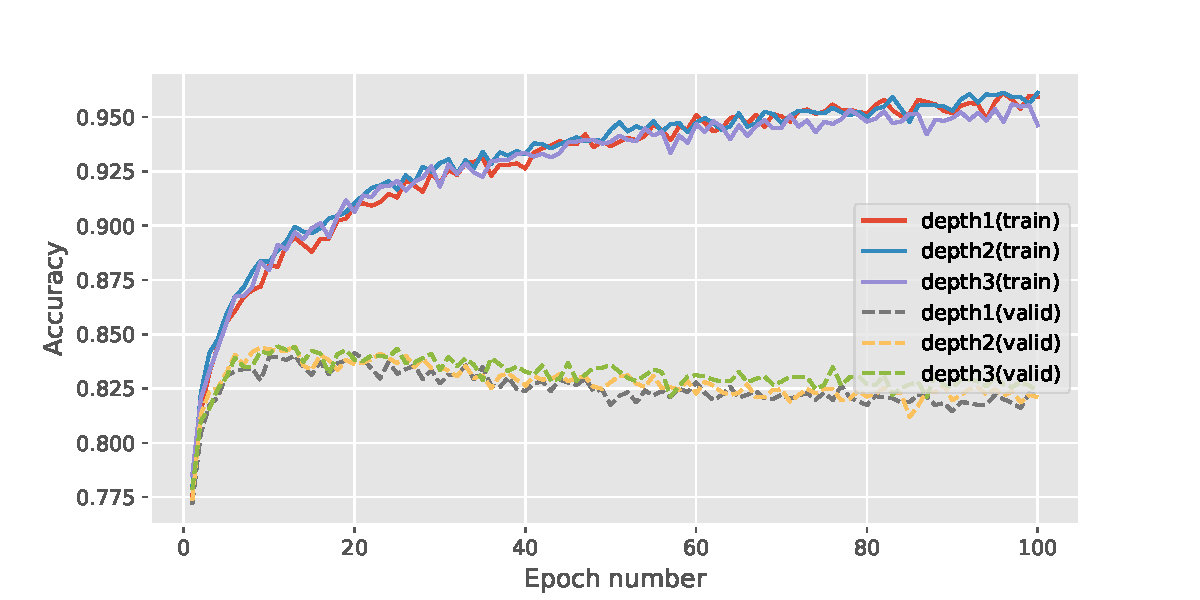
\includegraphics[width=\linewidth]{hidden_layer_acc.pdf}
        \caption{accuracy by epoch}
        \label{fig:depth_acccurves}
    \end{subfigure} 
    \begin{subfigure}{\linewidth}
        \centering
        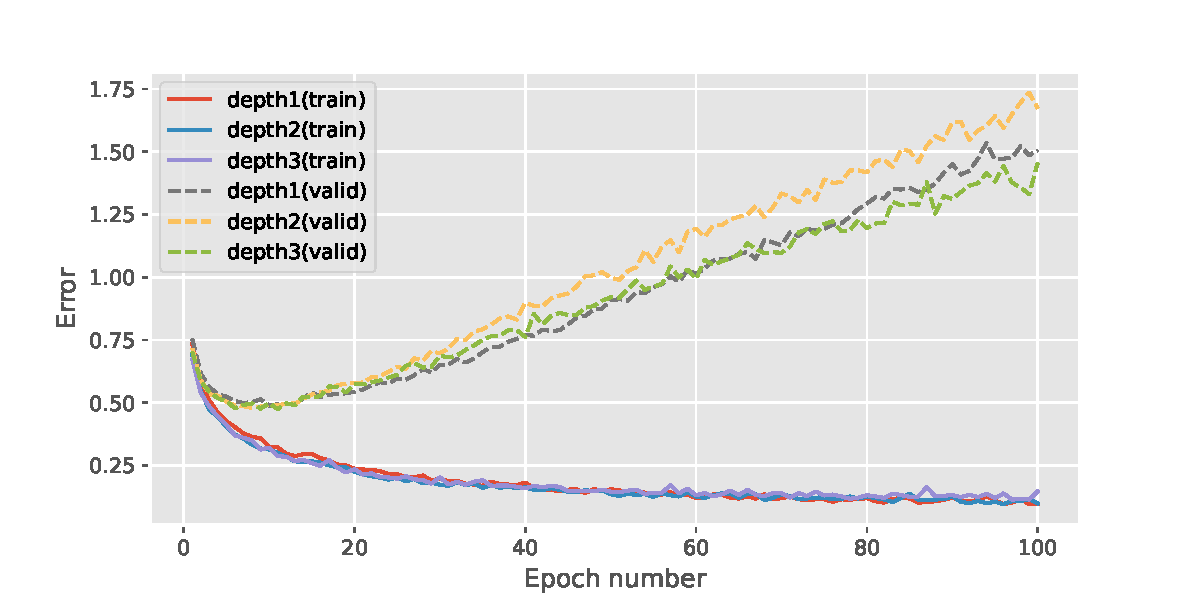
\includegraphics[width=\linewidth]{hidden_layer_err.pdf}
        \caption{error by epoch}
        \label{fig:depth_errorcurves}
    \end{subfigure} 
    \caption{Training and validation curves in terms of classification accuracy (a) and cross-entropy error (b) on the EMNIST dataset for different network depths.}
    \label{fig:depth}
\end{figure} 


}

%% Question Figure 4:
\newcommand{\questionFigureFour} {

\begin{figure*}[t]
    \centering
    \begin{subfigure}{.49\linewidth}
        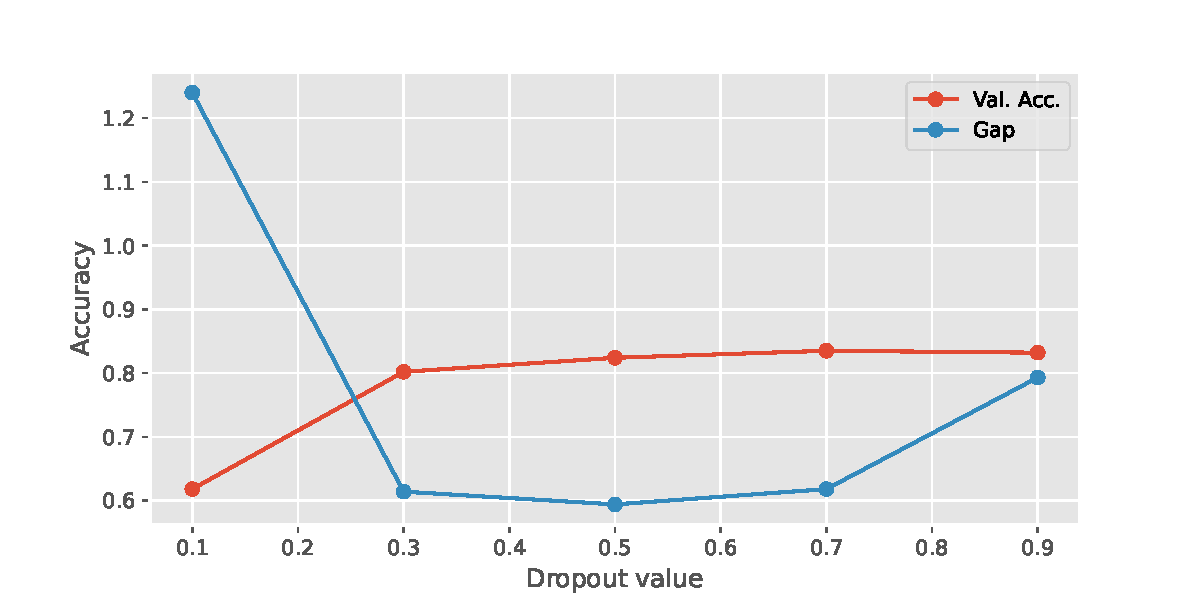
\includegraphics[width=\linewidth]{dropout.pdf}
        \caption{Metrics by dropout rate}
        \label{fig:dropoutrates}
    \end{subfigure} 
    \begin{subfigure}{.49\linewidth}
        \centering
        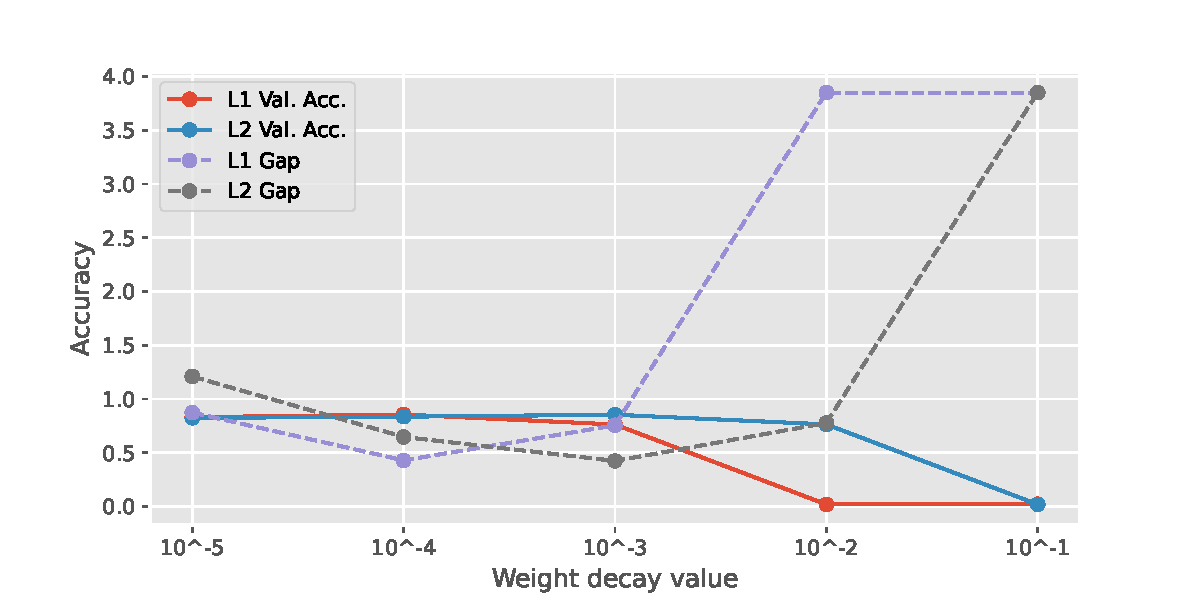
\includegraphics[width=\linewidth]{weightdecay.pdf}
        \caption{Metrics by weight penalty}
        \label{fig:weightrates}
    \end{subfigure} 
    \begin{subfigure}{\linewidth}
        \centering
        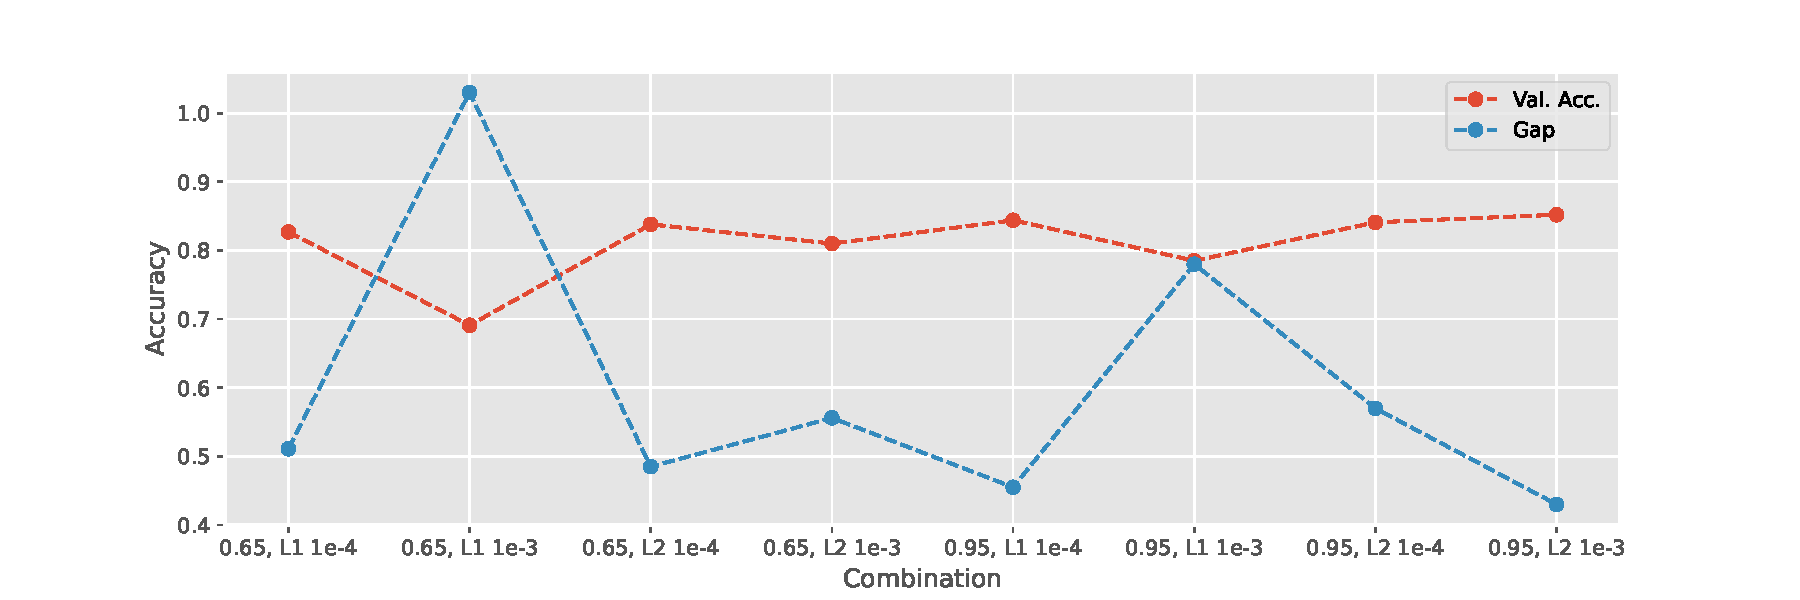
\includegraphics[width=\linewidth]{combination.pdf}
        \caption{Extra experiments}
        \label{fig:extra}
    \end{subfigure} 
    \caption{Hyperparameter search for every method and combinations}
    \label{fig:hp_search}
\end{figure*}


}

%% - - - - - - - - - - - - TABLES - - - - - - - - - - - - 

%% Question Table 1:

\newcommand{\questionTableOne} {


\begin{table}[t]
    \centering
    \begin{tabular}{c|cc}
    \toprule
        \# hidden units & val. acc. & generalization gap \\
    \midrule
         32       &     0.798        &    0.658                    \\
         64       &     0.813         &   0.768                    \\
         128      &     0.815        &    1.55                   \\ 
    \bottomrule
    \end{tabular}
    \caption{Validation accuracy (\%) and generalization gap (in terms of cross-entropy error) for varying network widths on the EMNIST dataset.}
    \label{tab:width_exp}
\end{table}
}


%% Question Table 2:
\newcommand{\questionTableTwo} {


\begin{table}[t]
    \centering
    \begin{tabular}{c|cc}
    \toprule
        \# hidden layers & val. acc. & generalization gap \\
    \midrule
         1          &     0.815       &     1.55                    \\
         2         &      0.818        &    1.73                    \\
         3               &      0.821      &    1.45                \\ 
    \bottomrule
    \end{tabular}
    \caption{Validation accuracy (\%) and generalization gap (in terms of cross-entropy error) for varying network depths on the EMNIST dataset.}
    \label{tab:depth_exps}
\end{table}

}

%% Question Table 3:
\newcommand{\questionTableThree} {


\begin{table*}[t]
    \centering
    \begin{tabular}{c|c|cc}
    \toprule
        Model    &  Hyperparameter value(s) & Validation accuracy & Generalization gap \\
    \midrule
    \midrule
        Baseline &  -                    &         0.821            &          1.45         \\
    \midrule
        \multirow{5}*{Dropout}
                 & 0.1                   &         0.618            &          1.24         \\
                 & 0.3                   &          0.802           &         0.614          \\
                 & 0.5                   &          0.824           &         0.594          \\
                 & \emph{0.7}            &      \emph{0.835}        &     \emph{0.618}       \\
                 & 0.9                   &          0.832           &         0.793          \\
    \midrule
        \multirow{5}*{L1 penalty}
                 & 1e-5                   &        0.831             &       0.874            \\
                 & \emph{1e-4}            &    \emph{0.855}          &   \emph{0.429}          \\
                 & 1e-3                   &        0.763             &       0.756            \\
                 & 1e-2                   &        0.020             &       3.850            \\
                 & 1e-1                   &        0.022             &       3.850            \\
    \midrule
        \multirow{5}*{L2 penalty}  
                 & 1e-5                   &       0.825              &      1.21             \\
                 & 1e-4                   &       0.836              &      0.647             \\
                 & \textbf{1e-3}            &   \textbf{0.854}           &  \textbf{0.424}          \\
                 & 1e-2                   &       0.764              &      0.778             \\
                 & 1e-1                   &       0.020              &      3.85             \\
    \midrule
        \multirow{8}*{Combined}  
                 & 0.65, L1 1e-4                 &         0.827            &       0.511            \\
                 & 0.65, L1 1e-3                 &          0.691           &       1.03            \\
                 & 0.65, L2 1e-4                   &        0.838             &     0.485              \\
                 & 0.65, L2 1e-3                  &         0.81            &       0.556            \\
                 &\emph{0.95, L1 1e-4}           &      \emph{0.844}        &    \emph{0.455}          \\
                 & 0.95, L1 1e-3                  &         0.758            &      0.78             \\
                 & 0.95, L2 1e-4                  &         0.841            &      0.570             \\
                 & 0.95, L2 1e-3                  &        0.852             &       0.430            \\
    \bottomrule
    \end{tabular}
    \caption{Results of all hyperparameter search experiments. \emph{italics} indicate the best results per series and \textbf{bold} indicate the best overall}
    \label{tab:hp_search}
\end{table*}


}

%% END of YOUR ANSWERS